\section{Analysis and Discussion}
\label{sec:analysis}


The preceding results establish that coordination broadly fails, that failures scale with complexity, and that agents accumulate partial information they cannot synthesize. 
We now investigate the mechanisms: first asking whether agents at least discover the \emph{right structural approach}, then tracing exactly where execution breaks down.

\subsection{Case Study: Emergent Coordination Patterns}

Figure~\ref{fig:heatmaps} visualizes the communication patterns that agents spontaneously adopt for three representative tasks. 
In the Global Max heatmap (Level-I, left), nearly all message traffic flows into column 0: Agent 0 emerges organically as a central aggregator, producing a near-perfect star topology. 
This self-organized structure closely matches the theoretically optimal pattern and yields high task success. 
In the Prefix Sum heatmap (Level-II, center), a prominent diagonal band reflects agents communicating primarily with their immediate neighbors, correctly capturing the sequential dependency of the prefix computation. 
However, off-diagonal scatter reveals that agents also broadcast beyond their neighbors, generating redundant overhead rather than the clean chain the task requires. 
In the Distributed Sort heatmap (Level-III, right), the matrix is uniformly dense: agents exchange messages with nearly every other agent, which is precisely what global data reorganization demands, yet the high density comes with highly uneven per-agent loads, and some senders dominate entire rows, suggesting uncoordinated flooding rather than structured exchange.




\begin{figure*}[t]
    \centering
    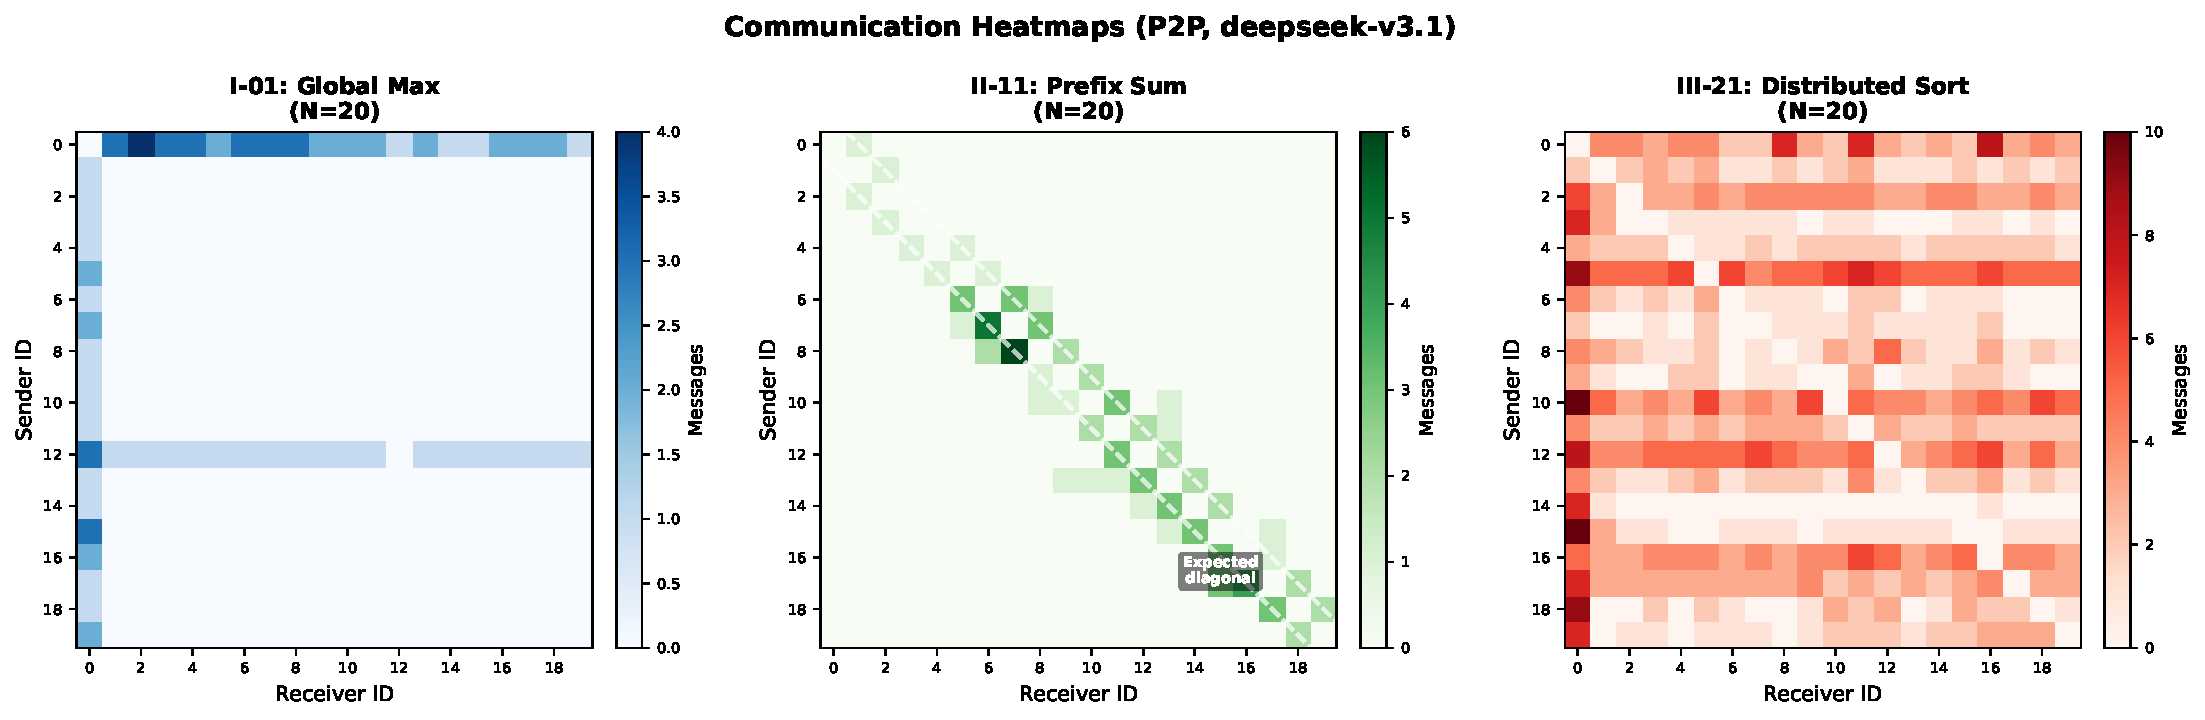
\includegraphics[width=1.0\textwidth]{figures/figure4_level_comparison.pdf} 
    \caption{Communication heatmaps for representative tasks with $N=20$ agents using DeepSeek-V3.1. 
    \textbf{Left}: I-01 (Global Max) shows emergent leader pattern. 
    \textbf{Center}: II-11 (Prefix Sum) exhibits diagonal pattern indicating partial spatial locality discovery. 
    \textbf{Right}: III-21 (Distributed Sort) shows dense all-to-all communication.}
    \label{fig:heatmaps}
\end{figure*}



Taken together, these patterns confirm that agents can translate high-level task descriptions into broadly appropriate coordination topologies without explicit instruction. 
Yet the heatmaps also reveal a consistent gap between structural intent and execution quality: even when the right topology emerges, agents over-communicate, distribute load unevenly, or fail to adhere to the optimal pattern. 
This raises the core question addressed next: given that agents communicate in approximately the right way, why do they still so often fail?

\subsection{The Communication-Reasoning Gap}

To classify failure systematically, we apply a two-stage hybrid procedure: rule-based detection identifies \textit{Premature Submission} (agent submits before reaching the task-specific minimum peer count), \textit{Consensus Failure} ($|\{\hat{y}_i\}_{i=1}^N| > 1$), and \textit{Computation Error} (full data receipt confirmed in log but answer incorrect). 
Two independent annotators then reviewed stratified runs, achieving Cohen's $\kappa = 0.87$; disagreements were resolved by discussion.

Analyzing execution logs under this scheme, we identified three distinct failure modes (Table~\ref{tab:failure_modes}). 
\textit{Premature Submission} (37.2\%) is the most prevalent: agents submit before gathering sufficient information---Agent-77 in Task I-06, for instance, submitted after contacting only 28 of 100 agents, yielding answer 208 vs.\ the expected 114. 
\textit{Consensus Failure} (29.9\%) occurs when agents communicate actively but cannot converge; one 100-agent XOR checksum run produced 12 distinct answers, with 86 agents converging on 146 while the remainder submitted values ranging from 42 to 238. 
\textit{Computation Error} (28.6\%) arises when agents collect all required data yet compute incorrectly, such as submitting 619 instead of 620 due to an off-by-one error during final aggregation. 
These modes frequently co-occur: 67 runs exhibit both Premature Submission and Consensus Failure, as early exits prevent subsequent consensus-building and widen the convergence gap for remaining agents.



Together, these three modes define the \textit{Communication-Reasoning Gap}: agents exhibit proficiency in the social mechanics of coordination---formatting messages, responding to peers, organizing information flow---while failing at the computational core of determining information sufficiency and synthesizing distributed state. 
This is not a failure of effort: behavioral comparison shows successful runs complete in fewer rounds, while verification behaviors appear in over 95\% of runs regardless of outcome. The bottleneck is reasoning quality at the integration stage, not communication intent.

\subsection{Implications and Future Directions}

The analyses jointly reveal a structural asymmetry with practical consequences. Coordination overhead does not merely reduce parallelization gains.
For Level-III tasks at $N{\geq}50$, it eliminates them entirely, leaving a coordinated team outperformed by a single agent with full data access. 
Perhaps most counterintuitively, spontaneous leader emergence which is conventionally assumed to help, actively hurts performance on Level-III tasks, because the aggregator becomes overwhelmed by the volume of global data it must process.

Three directions follow. 
First, agents need mechanisms to detect information sufficiency before committing to a final answer. 
Second, the explicit synchronization checkpoints present in successful runs should be formalized as consensus protocols. 
Third, adaptive protocol selection based on task structure could unlock model-protocol co-optimization, given the model-dependent affinities observed. \silobench{} provides the evaluation foundation for tracking progress along all three.


\begin{table}[t]
\centering
\small
\begin{tabular}{lcc}
\toprule
\textbf{Failure Mode} & \textbf{Count} & \textbf{Percent} \\
\midrule
Success & 153 & 50.8\% \\
Premature Submission & 112 & 37.2\% \\
Consensus Failure & 90 & 29.9\% \\
Computation Error & 86 & 28.6\% \\
\bottomrule
\end{tabular}
\caption{Failure mode distribution (categories not mutually exclusive).}
\label{tab:failure_modes}
\vspace{-0.3cm}
\end{table}


